\chapter{Estado da Arte} \label{cap:eda}
%2345678901234567890123456789012345678901234567890123456789012345678901234567890

Preliminarmente...

Falar aqui o que é ontologia, porque isso é importante e como jogos ou a
industria de entretenimento pode ver isso como util.

\section{Modelo Cognitivo Emocional} \label{cap:eda:mce}

Explicar...

	que ha diversos modelos diferentes de afetividade;

	o que eh o modelo OCC e porque ele foi escolhido;

	projetos ``atuais'' utilizando esse modelo.

\todo{por enquanto isso aqui foi copiado so da dissertacao e largado aqui...
reescrever!}
Segundo \citet{scherer2000tnoe}, na psicologia há diferentes modelos para
tentar mapear a afetividade: dimensionais, discretos, baseados em significados
e componentes. Os modelos dimensionais procuram estabelecer eixos de classes
de emoções e formas de se mover por esses.  Enquanto os modelos discretos
visam descrever um conjunto básico de emoções ou, ainda, um sistema adaptativo
que evolua a partir de um determinado ponto.  Os modelos baseados em
significados constroem estruturas semânticas e descrevem verbalmente o que
ocorre em determinado sentimento; em outras palavras, preocupa-se com as
situações em que ocasionaram o mesmo. Já os modelos baseados em componentes
entendem que emoções são aprendidas e, sendo assim, estudam o elo entre os
sentimentos e os eventos ou situações que as mesmas acontecem. Esse elo é
montado pela pessoa de diferentes formas.

\citet{Pic98} chama atenção que as emoções sempre foram consideradas um
estigma pela ciência que é fundamentalmente racional com hipóteses testáveis,
argumentos lógicos e experimentos repetitivos.  Entretanto, estudos
neurológicos recentes \cite{ledoux1998emotional,damasio2004erro} mostram a
importância das emoções na tomada de decisão.  \citet{damasio2004erro}
diferencia emoção de sentimento; para ele emoção é um estado físico do corpo e
sentimento é a percepção da mudança desse estado corporal.

\begin{figure*}
  \centering
    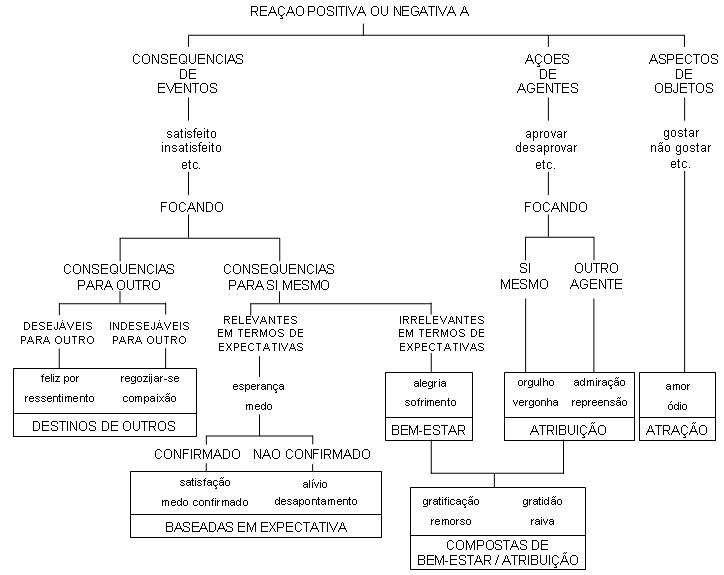
\includegraphics[width=150mm]{figuras/pontarolo_occ.png}
  \caption{Modelo OCC adaptado de \cite{pontarolo2008modelagem}.}
  \label{fig:occ_model}
\end{figure*}

O modelo proposto por \citeauthor*{ortony1988cse} \cite{ortony1988cse},
conhecidos na comunidade de Inteligência Artificial, é chamado de OCC por
causa de seus autores.  Esse modelo é classificado como baseado em
significados por descrever as situações de ocorrências de cada uma de suas 22
emoções.  Essas emoções são divididas em formas de se perceber o mundo a sua
volta: Eventos (importantes para alguma meta), Agentes (incluindo a si mesmo)
e Objetos (atração ou repulsa). Assim sendo, essas maneiras de se perceber o
mundo refletem diferentes jeitos de se analisar as situações que podem ser
relativas aos objetivos, valores morais ou gostos da pessoa.

A Figura~\ref{fig:occ_model} resume o modelo OCC e mostra as
percepções possíveis de um indivíduo.  Partindo da direita para esquerda, o
ramo mais básico, Aspectos de Objetos, é ativado quando se avalia o gosto de
alguém para algum objeto (inanimado ou não), por exemplo, alguém gostar de
rosas vermelhas.  No seguinte, Ações de agentes, o julgamento das ações
exercidas por outro indivíduo é realizado baseado nos valores morais da pessoa
que está julgando.  Sendo assim, por exemplo, reprovar a atitude de um colega
que ``colou'' na prova. O último da árvore, mais a esquerda, é o de evento que
representa as coisas que aconteceram (e foram consideradas importantes),
acontecem e acontecerão (objetivos almejados). Esses são avaliados segundo as
suas consequências para o alcance ou impedimento dos objetivos de uma pessoa.
Por exemplo, preciso ir bem no concurso para ficar satisfeito porque esse
evento me permitirá alcançar minha meta de ser contratado.

Ainda segundo o modelo OCC, as emoções possuem intensidades. Entretanto, há
distinção entre a valência da emoção e a valência do sentimento. No modelo, um
indivíduo só possui o sentimento quando a intensidade da emoção ultrapassar um
determinado limite.  Essa intensidade é obtida por uma função matemática que
utiliza variáveis de dois tipos: local, que influencia as emoções em um ramo
específico; e global, que influencia todas as emoções do indivíduo.  Um
exemplo de variável local é o desejo, enquanto que um exemplo de variável
global é o senso de realidade.

\section{Ontologias Emocionais} \label{cap:eda:oe}

Aqui tem que ter pelo menos 5 ontologias explicadas;
%1
%2
%3
%4
%5


\section{Ontologias de Humanos Virtuais} \label{cap:eda:odhv}

Explicar...
	pq ela eh necessaria.
	pelo menos 2.
%1
%2
